% !TeX root = ../tfg.tex
% !TeX encoding = utf8

\chapter{Símplices y complejos simpliciales}

\section{Símplices}

Con la finalidad de generalizar estructuras como el triángulo y el tetraedro, 
a finales del siglo XIX nace un nuevo concepto: el símplice. Su simplicidad y 
propiedades lo convirtieron en una herramienta muy versátil en el estudio de la
topología algebraica, dando lugar a lo que hoy conocemos como homología simplicial. 
En esta sección definiremos lo que es un símplice y algunos conceptos asociados a él
que nos serán de gran utilidad en el estudio de dicho campo.

\begin{definicion}
	Sea $\{a_0, \dots, a_n\}$ un conjunto de puntos en $\mathbb{R}^N$. 
	Diremos que dicho conjunto es \textbf{afínmente independiente} si 
	para cualesquiera $t_i \in \mathbb{R}$, las ecuaciones
	\[ \sum_{i=0}^{n}t_i=0 \quad \text{y} \quad \sum_{i=0}^{n}t_ia_i=0 \]
	implican que $t_0 = t_1 = \dots = t_n$.
\end{definicion}

\begin{definicion}
	Sea $\{a_0, \dots, a_n\}$ un conjunto de puntos afínmente independiente en 
	$\mathbb{R}^N$. Definimos el \textbf{símplice} $\sigma = [a_0, \dots, a_n]$ 
	generado por $a_0, 	\dots, a_n$ como el conjunto de todos los $x \in \mathbb{R}^N$ 
	tales que
	\[ x=\sum_{i=0}^{n}t_ia_i \quad \text{y} \quad \sum_{i=0}^{n}t_i=1 \]
	con $t_i \geq 0$, $i \in \{1, \dots, n\}$.
\end{definicion}
Los coeficientes $t_i$ están determinados de manera única por el punto $x$. A los términos  
$t_0, \dots, t_n$ los llamamos las \textbf{coordenadas baricéntricas} de $\sigma$
con respecto a $a_0, \dots, a_n$.

Los puntos $a_0, \dots, a_n$ que generan $\sigma$ los llamaremos \textbf{vértices} de $\sigma$
y al número $n$ lo llamaremos la \textbf{dimensión} de $\sigma$.

\begin{definicion}
	Sea $\sigma=[a_0, \dots, a_n]$ un símplice. Una \textbf{cara} de $\sigma$ será cualquier
	símplice generado por un subconjunto de $\{a_0, \dots, a_n\}$.
\end{definicion}
En particular, la cara de $\sigma$ generada por $a_0, \dots, a_{i-1}, a_{i+1}, \dots, a_n$ la 
llamamos la \textbf{cara opuesta} de $a_i$, $i \in \{0, \dots, n\}$. Las caras de $\sigma$ 
diferentes de $\sigma$ diremos que son \textbf{caras propias} de $\sigma$ y la unión de todas ellas la 
llamaremos el \textbf{borde} de $\sigma$. Finalmente, definimos el \textbf{interior} de $\sigma$
como el conjunto de puntos de $\sigma$ que no pertenecen a su borde.

\begin{ejemplo}
\begin{figure}[h]
	\begin{minipage}{.24\textwidth}
		\centering
		{
			\begin{tikzpicture}
				% 0-símplex
				\draw (0,0);
			\end{tikzpicture}
		}\subcaption{0-símplex}
	\end{minipage}
	\begin{minipage}{.24\textwidth}
		\centering
		{
			\begin{tikzpicture}
				% 1-símplex
				\draw (0,0) -- (1,0);
			\end{tikzpicture}
		}\subcaption{1-símplex}
	\end{minipage}
	\begin{minipage}{.24\textwidth}
		\centering
		{
			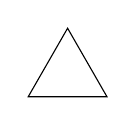
\begin{tikzpicture}
				% 2-símplex
				\draw (0,0) -- (1,0) -- (0.5,0.87) -- cycle;
			\end{tikzpicture}
		}\subcaption{2-símplex}
	\end{minipage}
	\begin{minipage}{.24\textwidth}
		\centering
		{
			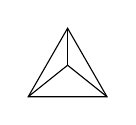
\begin{tikzpicture}
				% 3-símplex
				\draw (0,0) -- (1,0) -- (0.5,0.87) -- cycle;
				\draw (0.5,0.4) -- (0.5,0.87);
				\draw (0.5,0.4) -- (0,0);
				\draw (0.5,0.4) -- (1,0);
			\end{tikzpicture}
		}\subcaption{3-símplex}
	\end{minipage}
	\caption{Símplices en columnas}
\end{figure}
\end{ejemplo}

\section{Complejos simpliciales}

\begin{definicion}
	Un \textbf{complejo simplicial} $K$ en $\mathbb{R}^N$ es una colección de símplices en $\mathbb{R}^N$
	 tal que:
	\begin{enumerate}
		\item Toda cara de un símplice de $K$ está en $K$.
		\item La intersección de cualesquiera dos símplices de $K$ es una cara 
		de ambos símplices.
	\end{enumerate}
\end{definicion}

En ciertas ocasiones puede ser interesante saber si dada una colección cualquiera de símplices, esta es 
un complejo simplicial o no. Para ello, el siguiente lema nos puede ser de utilidad.

\begin{lema}
	Una colección $K$ de símplices es un complejo simplicial si, y sólo si, se cumplen las siguientes 
	condiciones:
	\begin{enumerate}
		\item Toda cara de un símplice de $K$ está en $K$.
		\item Los símplices de $K$ tienen interior disjunto dos a dos.
	\end{enumerate}
\end{lema}
\begin{proof}
	Primero, asumamos que $K$ es un complejo simplicial. MUNKRES
\end{proof}

\begin{definicion}
	Si $L$ es una subcolección del complejo simplicial $K$ que contiene todas las caras de sus 
	elementos, entonces $L$ es un complejo simplicial que llamaremos \textbf{subcomplejo} de $K$.
\end{definicion}
Entre los subcomplejos de un complejo simplicial, cabe destacar el siguiente. Diremos \textbf{p-esqueleto} 
de $K$ al subcomplejo formado por todas las caras de $K$ cuya dimensión sea menor o igual que $p$. Lo denotaremos por $K^{(p)}$. En particular, $K^{(0)}$ es el conjunto de vértices de $K$.

\begin{definicion}
	Sea $K$ un complejo simplicial de $\mathbb{R}^N$. Definimos el \textbf{politopo} de $K$ como el 
	subconjunto $|K| \subset \mathbb{R}^N$ tal que $|K|$ es la unión de todos los símplices de $K$.
\end{definicion}
Dotando a cada símplice de la topología inducida por la topología usual de $\mathbb{R}^N$, vamos a dotar ahora a $|K|$ de una topología. Diremos que un subconjunto $A \subset |K|$ es cerrado en $|K|$ si, y sólo si, $A \cap \sigma$ es cerrado en $\sigma$ para todo $\sigma \in K$. Si llamamos $T$ a la topología 
definida de esta forma, podemos ver fácilmente que $(|K|, T)$ es un espacio topológico. Claramente, $\emptyset, |K| \in T$. SEGUIR DEMOSTRANDO

Llamaremos \textbf{poliedro} a cualquier espacio topológico que sea el politopo de un complejo simplicial.

TAL VEZ ALGUNAS PROPIEDADES LOCALMENTE COMPACTO Y EJEMPLO

\section{Aplicaciones simpliciales}

Cuando trabajemos con complejos simpliciales, será interesante tener en cuenta cuándo las 
transformaciones entre ellos pueden ser continuas o incluso homeomorfismos. 

\begin{lema}
	Sean $K$ y $L$ dos complejos simpliciales y sea $f: K^{(0)} \rightarrow L^{(0)}$ una aplicación. 
	Supongamos que siempre que los vértices $v_0, \dots, v_n$ de $K$ generen un símplice en $K$, 
	los puntos $f(v_0), \dots, f(v_n)$ son vértices de un símplice de $L$. Entonces podemos extender $f$ 
	a una aplicación continua $g:|K| \rightarrow |L|$ tal que
	\[ x = \sum_{i=0}^{n}t_iv_i \quad \implies \quad g(x) = \sum_{i=0}^{n}t_if(v_i) \]
\end{lema}
Llamaremos a $g$ la \textbf{aplicación simplicial} (lineal) inducida por $f$.
\begin{proof}
	Por hipótesis, los vértices $f(v_0), \dots, f(v_n)$ generan un símplice $\tau$ en $L$. Por 
	ser $K$ un complejo simplicial, la suma de sus coeficientes $t_i$, con $i \in \{0, \dots, n\}$,  
	es igual a uno, luego $g(x) = \sum_{i=0}^{n}t_if(v_i)$ es un punto de $\tau$. Podemos ver que 
	$g$ es una aplicación continua del símplice $\sigma$ generado por $v_0, \dots, v_n$ al símplice 
	$\tau$ generado por $f(v_0), \dots, f(v_n)$.
	
	Ahora tan solo nos queda ver que $g:|K| \rightarrow |L|$ es continua. Bien, pues por ser 
	$g: \sigma \rightarrow \tau$ continua, también lo es $g: \sigma \rightarrow |L|$. Finalmente 
	por el lema METER LEMA ANTERIOR 2.3 DE MUNKRES, $g:|K| \rightarrow |L|$ es continua.
\end{proof}

\begin{lema}\label{lem:homeo_complex}
	Supongamos que $f:K^{(0)} \rightarrow L^{(0)}$ es una aplicación biyectiva tal que los vértices 
	$v_0, \dots, v_n$ de $K$ generan un símplice de $K$ si, y sólo si, $f(v_0), \dots, f(v_n)$ 
	generan un símplice de $L$. Entonces la aplicación simplicial inducida $g:|K| \rightarrow |L|$ 
	es un homeomorfismo.
\end{lema}
Diremos entonces que $g$ es un \textbf{homeomorfismo simplicial} de $K$ con $L$.
\begin{proof}
	Por hipótesis, cada símplice $\sigma \in K$ se identifica con otro símplice $\tau \in L$. 
	Por tanto, debemos comprobar que la aplicación lineal $h: \tau \rightarrow \sigma$ inducida por 
	la correspondencia de vértices $f^{-1}$ es la inversa de $g: \sigma \rightarrow \tau$. Si 
	consideramos $x = \sum_{i=0}^{n}t_i v_i$, entonces por definición $g(x) = \sum_{i=0}^{n}t_if(v_i)$.
	Luego
	\[ h(g(x)) = h(\sum_{i=0}^{n}t_if(v_i)) = \sum_{i=0}^{n}t_i f^{-1}(v_i) = \sum_{i=0}^{n}t_i v_i = x \]
	
\end{proof}

\section{Complejos simpliciales abstractos}

Si bien la definición actual de los complejos simpliciales puede llegar a ser de gran utilidad, en 
la práctica muchas veces no es necesario usar las herramientas que nos proporciona la geometría afín. 
Es por ello que vamos a introducir una descripción puramente combinatoria de los complejos simpliciales 
que, aun siendo más simples, son de gran utilidad a la hora de trabajar con espacios topológicos.

\begin{definicion}
	Un \textbf{complejo simplicial abstracto} (o simplemente complejo abstracto) es una 
	colección $\mathcal{S}$ de conjuntos finitos no vacíos tal que si $A \in \mathcal{S}$, 
	entonces para todo $B \subset A$ con $B$ no vacío, $B \in \mathcal{S}$.
\end{definicion}

Al elemento $A$ de $\mathcal{S}$ lo llamaremos \textbf{símplice} de $A \in \mathcal{S}$. La 
\textbf{dimensión} de $A$ es una menos que el número de elementos que le pertenecen. Todo 
subconjunto de $A$ lo llamaremos \textbf{cara} de $A$. En cuanto a la \textbf{dimensión} de 
$\mathcal{S}$, diremos que es igual al máximo de las dimensiones de sus elementos o en caso de 
no haberlo, diremos que la dimensión de $\mathcal{S}$ es infinita. El \textbf{conjunto de vértices} 
$V$ de $\mathcal{S}$ diremos que es la unión de elementos de $\mathcal{S}$ que contienen un único punto. 
Llamaremos \textbf{subcomplejo} de $\mathcal{S}$ a cualquier subcolección de $\mathcal{S}$ que sea 
un complejo simplicial abstracto en sí.

Sean $V_S$, $V_T$ los conjuntos de vértices de los complejos abstractos $\mathcal{S}$, $\mathcal{T}$  respectivamente. Dos complejos abstractos $\mathcal{S}$ y $\mathcal{T}$ diremos que son 
\textbf{isomorfos} si existe una aplicación biyectiva $f: V_S \rightarrow V_T$ tal que 
$\{a_0, \dots, a_n\} \in \mathcal{S}$ si, y sólo si, $\{f(a_0), \dots, f(a_n)\} \in \mathcal{T}$.

\begin{definicion}
	Sean $K$ un complejo simplicial y $V$ su conjunto de vértices. Sea $\mathcal{K}$ la colección de 
	todos los subconjuntos $\{a_0, \dots, a_n\} \subset V$ tales que los vértices $a_0, \dots, a_n$ 
	generan un símplice de $K$. Entonces llamaremos a la colección $\mathcal{K}$ el 
	\textbf{esquema de vértices} de $K$.
\end{definicion}

Después de realizar todas las definiciones pertinentes, ya estamos en condiciones de enunciar el 
siguiente teorema.

\begin{teorema}
	Las siguientes afirmaciones son ciertas:
	\begin{enumerate}[label=(\alph*)]
		\item Todo complejo abstracto $\mathcal{S}$ es isomorfo al esquema de vértices de algún 
		complejo simplicial $K$.
		\item Dos complejos simpliciales son linealmente isomorfos si, y sólo si, sus esquemas 
		de vértices son isomorfos como complejos simpliciales abstractos.
	\end{enumerate}
\end{teorema}
\begin{proof}
	Para demostrar $(a)$, empezaremos tomando un conjunto de índices $J$. Llamemos $\mathbf{E}^J$ 
	al subconjunto de funciones $x: J \rightarrow \mathbb{R}$ de $\mathbb{R}^J$ tales que $x(\alpha) = 0$ 
	para todo $\alpha \in J$ excepto para un número finito de valores. Sea $\Delta^J$ la 
	colección de todos los símplices en $\mathbf{E}^J$ generados por subconjuntos finitos de 
	la base usual de $\mathbf{E}^J$. $\Delta^J$ es un complejo simplicial. 
	Sean entonces $\sigma, \tau$ símplices de $\Delta^J$, la 
	unión de sus conjuntos de vértices es afínmente independiente y genera un símplice en $\Delta^J$.
	Diremos que $\Delta^J$ es un \textit{símplice de dimensión infinita}.
	
	Sea ahora $\mathcal{S}$ un complejo abstracto con conjunto de vértices $V$. Tomamos un conjunto 
	de índices $J$ lo bastante grande para que podamos tomar una aplicación inyectiva 
	$f: V \rightarrow J$. A continuación, vamos a tomar un subcomplejo de $\Delta^J$ tal que para 
	cada símplice abstracto $\{a_0, \dots, a_n\} \in \mathcal{S}$, el símplice (geométrico) generado 
	por $f(a_0), \dots, f(a_n)$ está en $K$. Por tanto $K$ es un complejo simplicial y 
	$f$ es un isomorfismo entre $\mathcal{S}$ y el esquema de vértices de $K$.
	
	En cuanto a $(b)$, es una consecuencia inmediata del \autoref{lem:homeo_complex}
\end{proof}

\begin{definicion}
	Si el complejo simplicial abstracto $\mathcal{S}$ es isomorfo al esquema de vértices del 
	complejo simplicial $K$, diremos que $K$ es una \textbf{realización geométrica} de $\mathcal{S}$.
\end{definicion}

\begin{lema}
	Sea $\mathcal{S}$ un comlpejo simplicial abstracto de dimensión $d$. Entonces $\mathcal{S}$ tiene 
	una realización geométrica en $\mathbb{R}^{2d+1}$.
\end{lema}
\begin{proof}
	TENGO LA DEMOSTRACION EN TDA PERO HAY QUE BUSCAR OTRA FUENTE.
\end{proof}

\begin{ejemplo}
	ALGUN EJEMPLO QUE MUESTRE SU UTILIDAD.
\end{ejemplo}

\section{Triangulaciones}



\section{Algunos complejos simpliciales}

\endinput
%--------------------------------------------------------------------
% FIN DEL CAPÍTULO. 
%--------------------------------------------------------------------
